\subsection{Graph Operators and Eigenvalues}

We consider weighted, undirected graphs $G = (V, E)$ with vertices $V=
\{v_1,\cdots, v_N\}$ and edges $E \subseteq V \times V$. The weighted adjacency
matrix $A\in\BBR^{N\times N}$ has entries $a_{ij} > 0$ to give the weight of an
edge $(i,j) \in E$ and $a_{ij} = 0$ otherwise. The degree matrix $D\in\BBR^
{N\times N}$ is the diagonal matrix of weighted node degrees, i.e. $D_{ii} =
\sum_j a_{ij}$. Several of the matrices in spectral graph theory are defined in
terms of $D$ and $A$.  We describe a few of these below, along with their
connections to other research areas. For each operator, we let $\lambda_1 \leq
\ldots \leq \lambda_N$ denotes the eigenvalues in ascending order.

\paragraph{Adjacency Matrix: $\pmb{A}$}

Many studies on the spectrum of $A$ originate from random matrix theory where
$A$ represents a random graph model. In these cases, the limiting behavior of
eigenvalues as $N\To\infty$ is of particular interest. Besides the growth of
extremal eigenvalues~\cite{chung1997spectral}, Wigner's semicircular law is 
the most renowned result about the spectral distribution of the adjacency
matrix~\cite{wigner1958distribution}. When the edges are i.i.d.~random variables
with bounded moments, the density of eigenvalues within a range converges to a
semicircular distribution. One famous graph model of this type is the
\ErdosRenyi\ graph, where $a_{ij} = a_{ji} = 1$ with probability $p < 1$, and
$0$ with probability $1-p$. Farkas et al.~\cite{farkas2001spectra} has extended
the semicircular law by investigating the spectrum of scale-free and small-world
random graph models. They show the spectra of these random graph models relate
to geometric characteristics such as the number of cycles and the degree
distribution.

\paragraph{Laplacian Matrix: $\pmb{L = D - A}$}

The Laplace operator arises naturally from the study of dynamics in both
spectral geometry and spectral graph theory. The continuous Laplace operator
and its generalizations are central to the description of physical systems
including heat diffusion~\cite{mckean1972selberg}, wave propagation~
\cite{levy2006laplace}, and quantum mechanics~\cite{ducastelle1970moments}. It
has infinitely many non-negative eigenvalues, and Weyl's law~
\cite{weyl1911asymptotische} relates their asymptotic distribution to the volume
and dimension of the manifold. On the other hand, the discrete Laplace matrix
appears in the formulation of graph partitioning problems. If $f \in \{ \pm 1
\}^N$ is an indicator vector for a partition $V = V_+ \cup V_-$, then $f^T L
f/4$ is the number of edges between $V_+$ and $V_{-}$, also known as the cut
size. $L$ is a positive-semidefinite matrix with the vector of all ones as a
null vector. The eigenvalue $\lambda_2$, called the {\em algebraic
connectivity}, bounds from below the smallest bisecting cut size; $\lambda_2 =
0$ if and only if the graph is disconnected. In addition, eigenvalues of $L$
also appear in bounds for vertex connectivity ($\lambda_2$)~
\cite{cvetkovic2009introduction}, minimal bisection ($\lambda_2$)~
\cite{donath2003lower}, and maximum cut ($\lambda_N$)~\cite{trevisan2012max}.

\paragraph{Normalized Laplacian Matrix: $\pmb{\overline{L} = I - D^{-1/2}AD^
{-1/2}}$}

We will also mention the normalized adjacency matrix $\overline{A} =
D^{-1/2}AD^{-1/2}$ and graph random walk matrix $P = D^{-1}A$ here, because
these matrices have the same eigenvalues as $\bar{L}$ up to a shift. The
connection to some of the most influential results in spectral geometry is
established in terms of eigenvalues and eigenvectors of normalized Laplacian. A
prominent example is the extension of Cheeger's inequality to the discrete
case, which relates the set of smallest conductance $h(G)$ (the Cheeger
constant)  to the second smallest eigenvalue of the normalized Laplacian,
$\lambda_2(\overline{L})$~\cite{montenegro2006mathematical}:
\begin{equation}\label{eqn:cheeger}
  \lambda_2(\overline{L})/2\leq h(G) = \min_{S\subset V}\frac{\abs{\{(i,j)\in
  E, i\in S, j\notin S\}}}{\min(\text{vol}(S), \text{vol}(V\backslash S))} \leq 
  \sqrt{2\lambda_2(\overline{L})} ,
\end{equation}
where $\vol(S) = \sum_{i \in S}\sum_{j=1}^{N}a_{ij}$. Cheeger's inequality
offers crucial insights and powerful techniques for understanding popular
spectral graph algorithms for partitioning~\cite{mcsherry2001spectral} and
clustering~\cite{ng2002spectral}. It also plays a key role in analyzing the
mixing time of Markov chains and random walks on a graph
~\cite{Mihail-1989-Markov,Sinclair-1989-Markov}. For all these problems,
extremal eigenvalues again emerge from relevant optimization formulations.

\subsection{Spectral Density (Density of States --- DOS)}
Let $H\in\BBR^{N\times N}$ be any symmetric graph matrix with an
eigendecomposition $H = Q\Lambda Q^T$, where $\Lambda = \diag 
(\lambda_1,\cdots,\lambda_N)$ and $Q = [q_1,\cdots, q_N]$ is orthogonal. The
spectral density induced by $H$ is the generalized function
\begin{equation}\label{eqn:dos}
  \mu(\lambda) = \frac{1}{N}\sum_{i=1}^N \delta(\lambda - \lambda_i), \quad \int
  f(\lambda) \mu(\lambda) = \tr(f(H))
\end{equation}
where $\delta$ is the Dirac delta function and $f$ is any analytic test
function. The spectral density $\mu$ is also referred to as the \emph{density
of states} (DOS) in the condensed matter physics literature~
\cite{weisse2006kernel}, as it describes the number of states at different
energy levels. For any vector $u\in\BBR^N$, the local density of states (LDOS)
is
\begin{equation}\label{eqn:ldos}
  \mu(\lambda; u) = \sum_{i=1}^N|u^Tq_i|^2\delta(\lambda-\lambda_i), \quad \int
  f(\lambda)\mu(\lambda; u) = u^T f(H) u.
\end{equation}
Most of the time, we are interested in the case $u=e_k$ where $e_k$ is the $k$th
standard basis vector---this provides the spectral information about a
particular node. We will write $\mu_k(\lambda) = \mu(\lambda; e_k)$ for the
pointwise density of states (PDOS) for node $v_k$. It is noteworthy $|e_k^Tq_i|
= |q_i(k)|$ gives the magnitude of the weight for $v_k$ in the $i$-th
eigenvector, thereby the set of $\{\mu_k\}$ encodes the entire spectral
information of the graph up to sign differences. These concepts can be easily
extended to directed graphs with asymmetric matrices, for which the eigenvalues
are replaced by singular values, and eigenvectors by left/right singular
vectors.

Naively, to obtain the DOS and LDOS requires computing all eigenvalues and
eigenvectors for an $N$\hyp{}by\hyp{}$N$ matrix, which is infeasible for large
graphs. Therefore, we turn to algorithms that approximate these densities. Since
the DOS is a generalized function, it is important we specify how the estimation
is evaluated. One choice is to treat $\mu$ (or $\mu_k$) as a distribution, and
measure its  approximation error with respect to a chosen function space
$\calL$. For  example, when $\calL$ is the set of Lipschitz continuous functions
taking the value 0 at 0, the error for estimated $\widetilde{\mu}$ is in the
Wasserstein distance (a.k.a.\ earth-mover distance)~\cite{kantorovich1958space}
\begin{equation}\label{eqn:waisserstein}
W_1(\mu,\widetilde{\mu}) = \sup\Big\{\int (\mu(\lambda)-\widetilde{\mu}(\lambda
))f(\lambda)d\lambda : \text{Lip}(f)\leq 1\Big\}\,.
\end{equation}
This notion is particularly useful when $\mu$ is integrated against in 
applications such as computing centrality measures.

On the other hand, we can regularize $\mu$ with a mollifier $K_\sigma$ (i.e.,
a smooth approximation of the identity function):
\begin{equation}\label{eqn:reg_dos}
  (K_\sigma\ast\mu)(\lambda) = \int_\BBR \sigma^{-1} K\left(\frac{\lambda-\nu}{
  \sigma}\right)\mu(\nu)d\nu
\end{equation}
A simplified approach is numerically integrating $\mu$ over small intervals of
equal size to generate a spectral histogram. The advantage is the error is now
easily measured and visualized in the $L_\infty$ norm. For example, Figure 
\ref{fig:caida} shows the exact and approximated spectral histogram for the
normalized adjacency matrix of an Internet topology. 
\begin{figure}[ht]
  \begin{center}
    \begin{subfigure}{0.47\textwidth}
      \centering  
      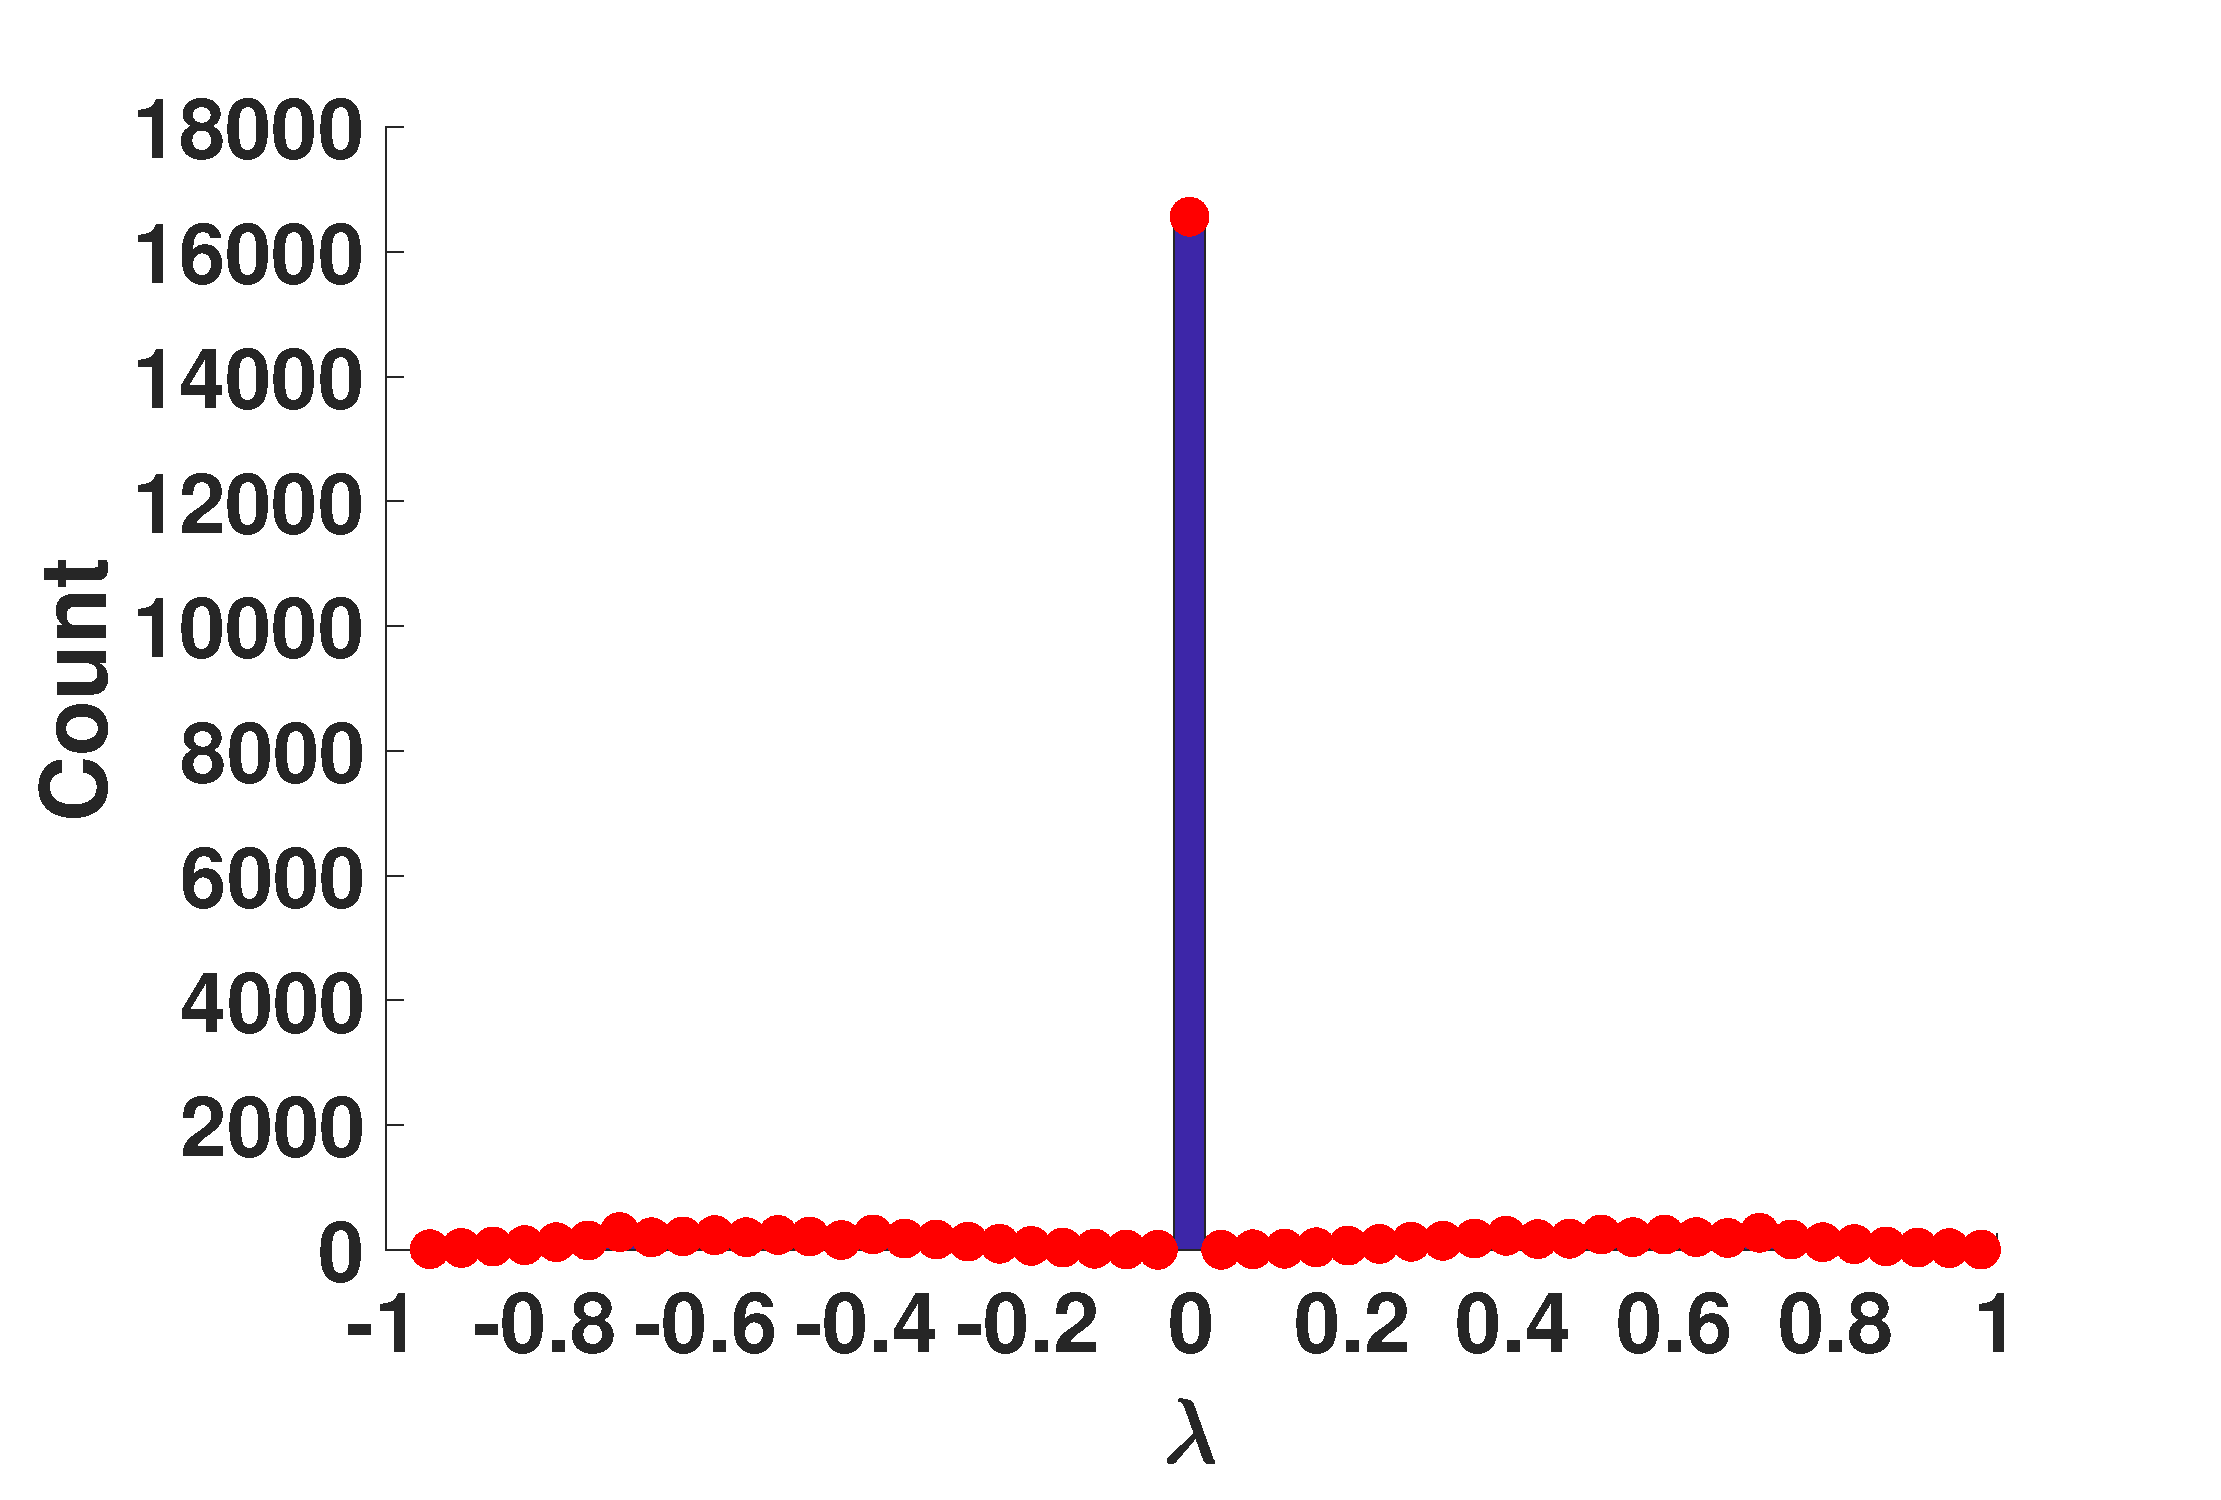
\includegraphics[width=\textwidth,trim = .4cm 0.5cm 3.5cm 1.3cm,clip]
      {./ndos/pics/as_caida_hist}
      \caption{Spectral Histogram}
      \label{fig:caida_full}
    \end{subfigure}
    %
    \begin{subfigure}{0.47\textwidth}
      \centering
      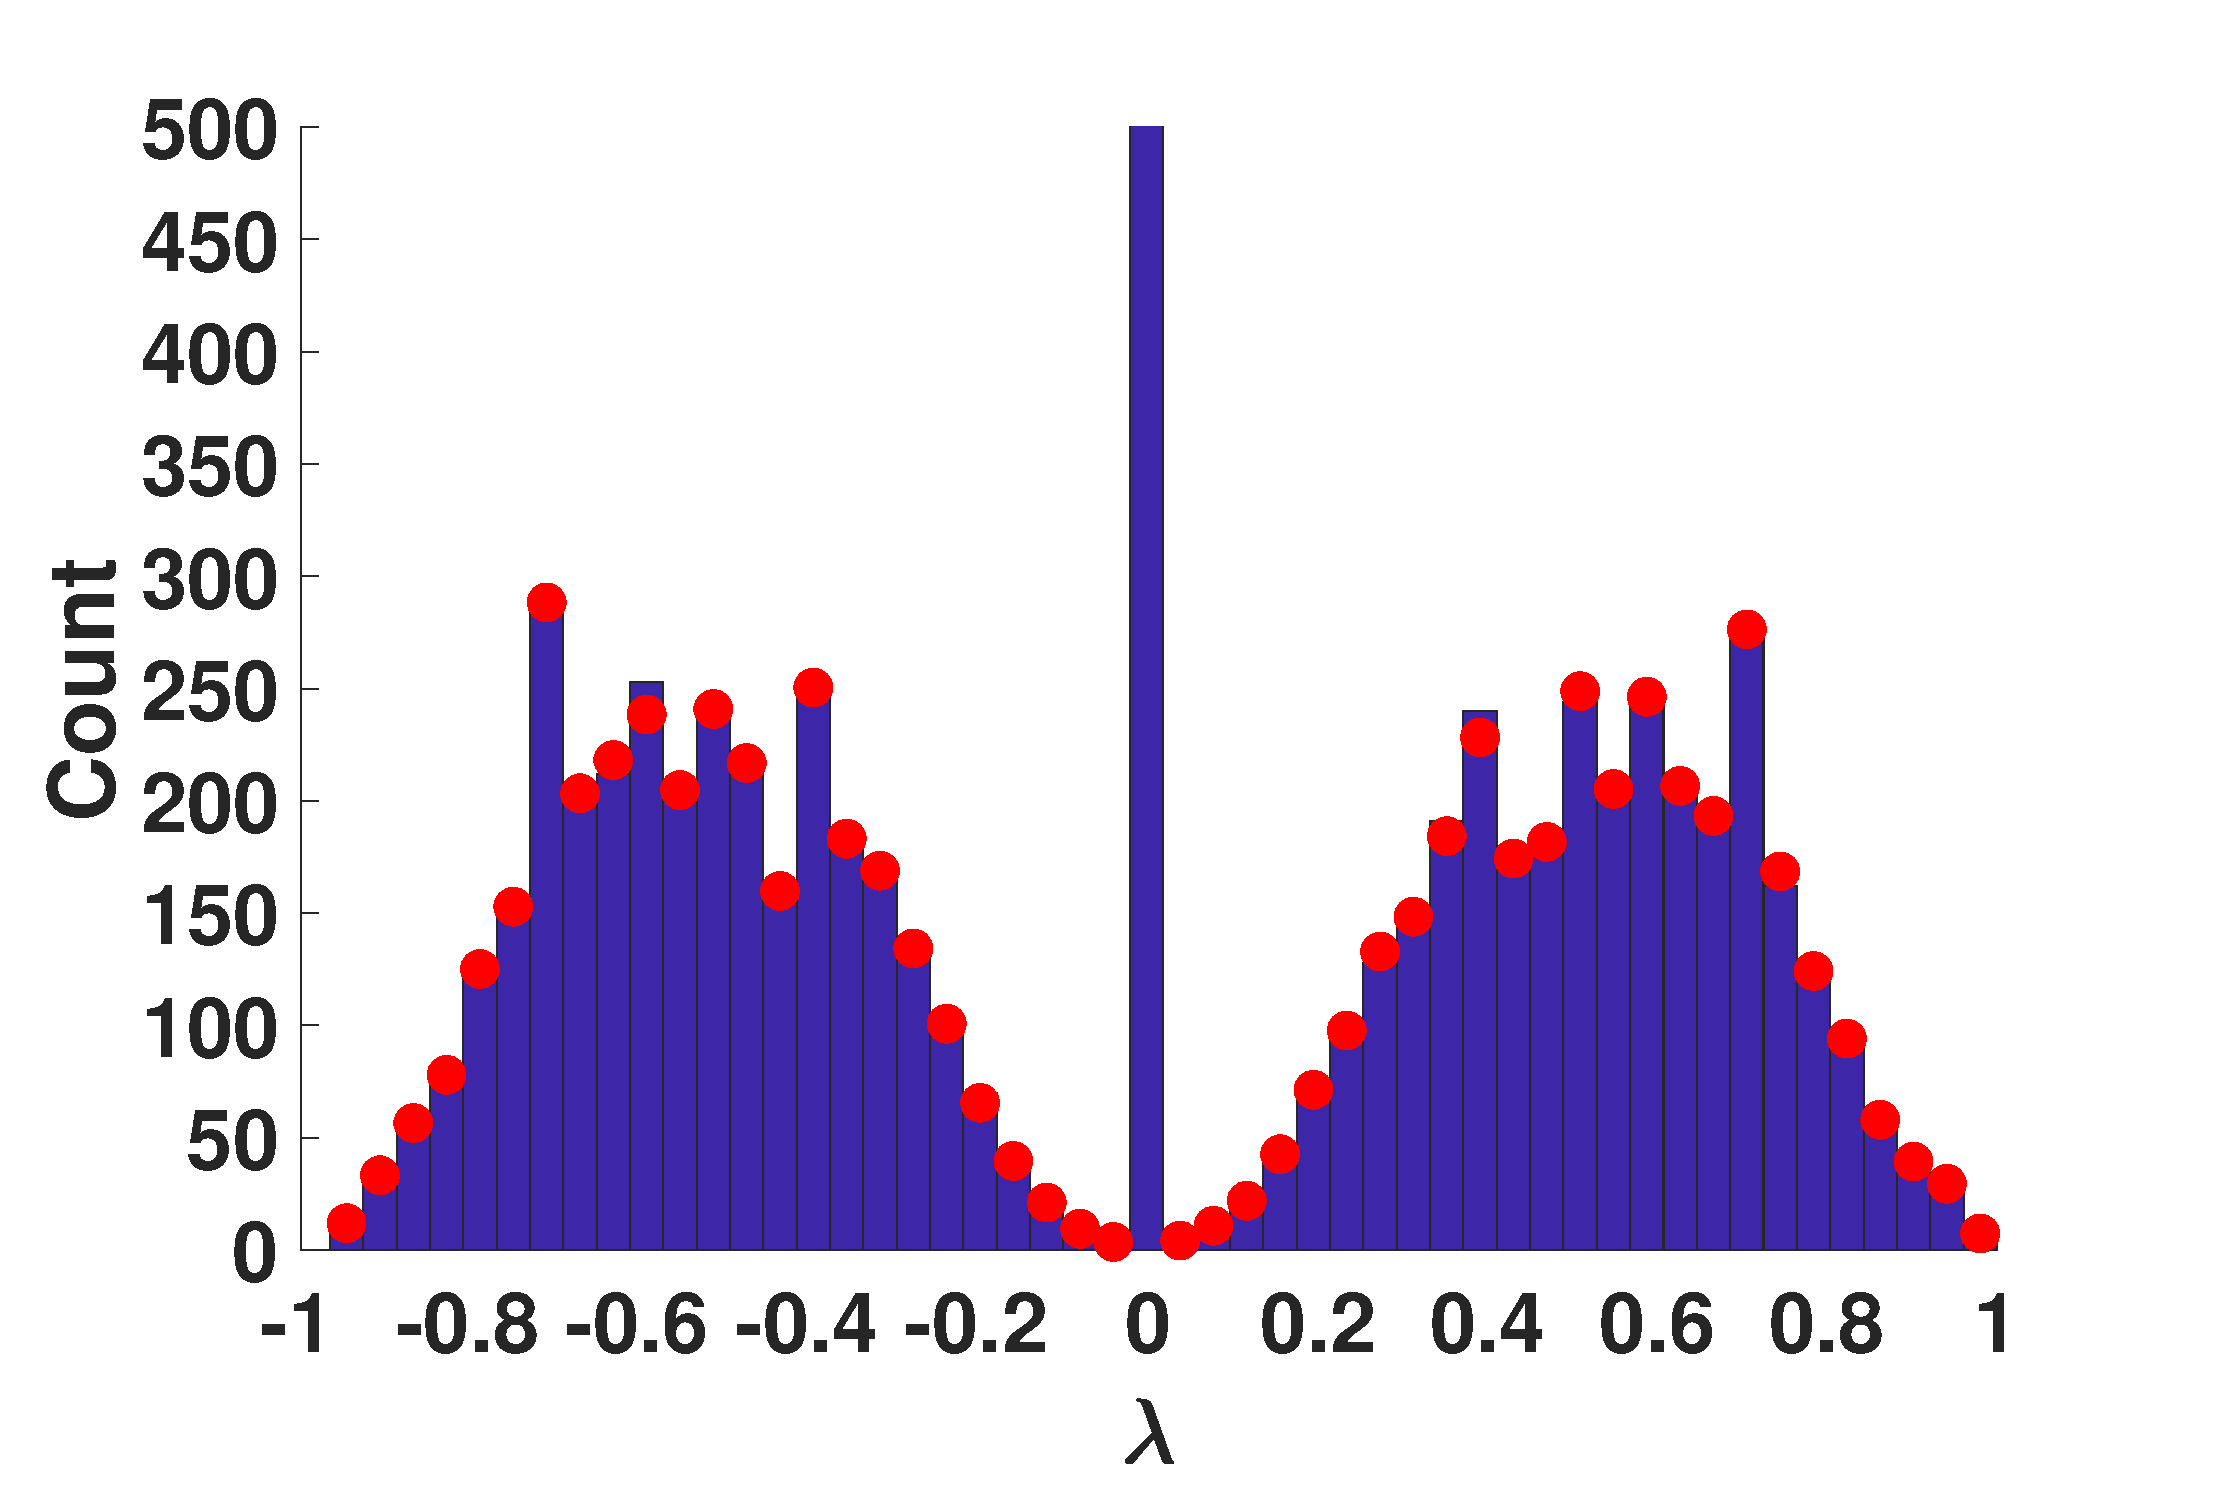
\includegraphics[width=\textwidth,trim = .4cm 0.5cm 3.5cm 1.3cm,clip]
      {./ndos/pics/as_caida_hist_zoom}
      \caption{Zoom-in View}
      \label{fig:caida_zoom}
    \end{subfigure}
    \caption{Spectral histogram for the normalized adjacency matrix for the
    CAIDA autonomous systems graph~\cite{caida2012}, an Internet topology with
    $22,965$ nodes and $47,193$ edges. Blue bars are the real spectrum, and red
    points are the approximated heights. (a) contains high multiplicity around
    eigenvalue $0$, so (b) zooms in to height between $[0,500]$.} 
    \label{fig:caida}
  \end{center}
\end{figure}
\vspace{-.5cm}